\chapter{Methodology}

\todo{Brief overview over the approach}

\section{Dataset used in analysis}

\todo{Add flowchart over DB structure}

\subsection{Vessel position history}

\begin{itemize}
    \item Validated on geographical coordinates
    \item Validated on MMSI -> IMO mapping and valid values
    \item Filtered from 1 billion to 450 million etc...
    \item Visualization ?
\end{itemize}

MO-AIS-DB => IMO, MMSI mapping => positional validation => ML-DB

\subsection{Vessel transitions}

 - A direct copy of MO's

\subsection{Ports}

 - A direct copy of MO's "visible" ports

\subsection{Segments}

 - A direct copy of MO's


\section{Vessel voyage definition}

\begin{itemize}
    \item Transitions
    \item (Clustering)
\end{itemize}


\subsection{Transition voyages}

\begin{itemize}
    \item Extracting departure=>arrival times grouped by vessels, ordered by time
    \item Finding position reports between each timestamp for given vessel
    \item Constructing trajectory (3D trajectory with timestamps)
    \item Validating trajectory, noise filtering
\end{itemize}

\section{Machine Learning (ML) data preparation}

\subsection{Trajectory sampling}

\begin{itemize}
    \item Why? How?
    \item Sampling based on distance
    \item Sampling based on time
\end{itemize}

\subsection{\acrfull{mstd}}

\begin{figure}[htbp]  % order of priority: h here, t top, b bottom, p page
    \centering
    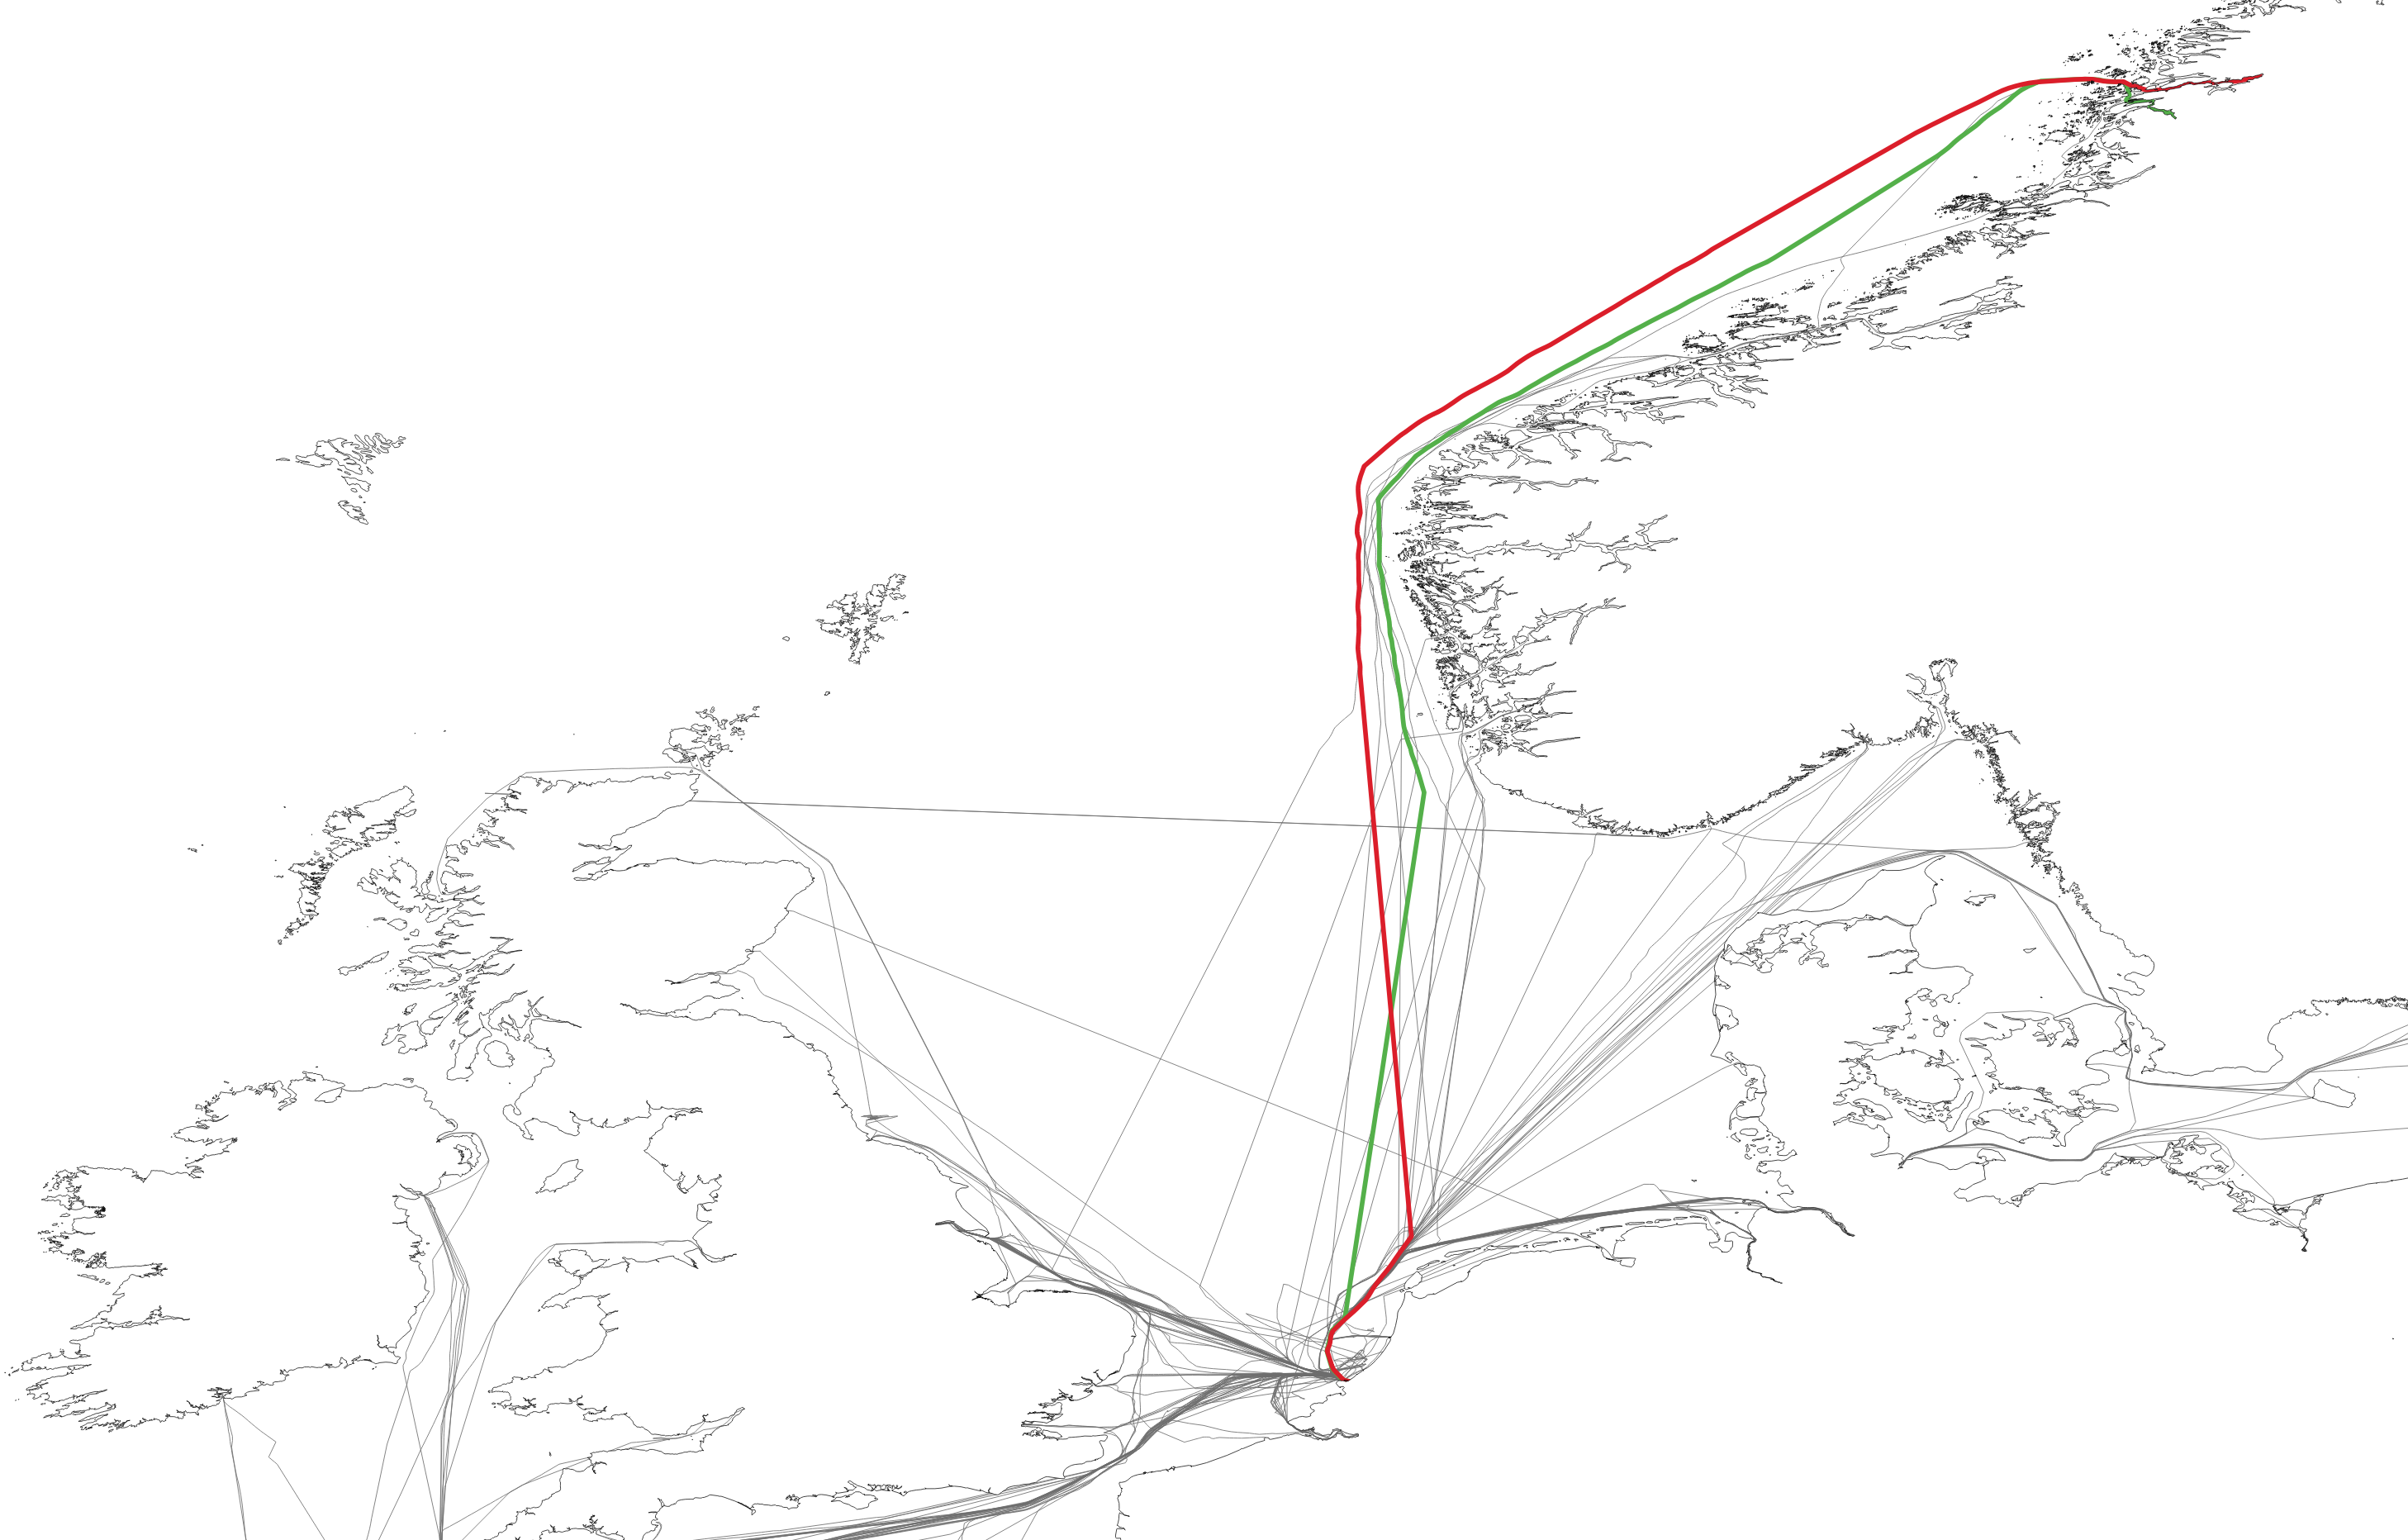
\includegraphics[width=1.0\textwidth]{figures/mstd}
    \caption{Example of \acrshort{mstd} for a given historical trajectory where the red line is the given trajectory and the green line is the most similar historical trajectory.}
    \label{fig:mstd}
\end{figure}


\subsection{Building ML data training set}

\begin{itemize}
    \item Batch calculating MSTD
    \item Different trajectory similarity approaches
    \item Adding more data attributes per voyage such as seasons, ballast/laden, etc\ldots
    \item Final result/structure
\end{itemize}

\subsection{Dataset imbalance}

\begin{itemize}
    \item Minority oversampling
    \item Majority undersampling
\end{itemize}

\subsection{Categorical label encoding}

\begin{itemize}
    \item Categorical values/labels must be encoded
    \item Label encoding vs one-hot encoding
\end{itemize}

\section{ML-based training and destination prediction}

\subsection{Model selection}

\begin{itemize}
    \item Tree-based classifiers
    \item Multi-layered perceptrons classifiers
    \item Support-vector machines
    \item Multi-class classifiers vs OneVsRest binary classifiers
\end{itemize}

\subsection{Configuration and parameter optimization}

\subsection{Training}

\subsection{Evaluation process and metrics}

\begin{itemize}
    \item X-Folder-cross-validation
    \item Metrics: F1, precission, recall, AUC, vs accuracy
    \item Computing performance?
    \item How fast is it to compute the next destination of every vessel in the world
\end{itemize}
